\section{Resultados}
    El dataset de imágenes está conformadas por algunas de las consideras 
    durante la revisión del código de este tema durante la clase. Se presentan 
    algunos de los resultados más relevantes de las imágenes transformadas 
    destacando cómo son modificadas o alteradas con las transformaciones 
    consideradas. Para observar de mejor manera las imágenes, se sugiere 
    referirse a la libreta de Jupyter (\href{https://github.com/alexisuaguilaru/ProcDigImg/blob/main/Proy03/proyecto.ipynb}{proyecto.ipynb}) 
    que cumple también con el propósito de mostrar una bitácora de experimentos.

    \subsection{Imagen 1 (Rotación)}
        En una de las imágenes donde más se puede apreciar la rotación es en 
        la de una flecha, empleando diferentes ángulos se aprecia como la forma 
        y contorno de la figura no son degradas por aplicarle una rotación. 

        \begin{figure}[H]
            \centering
            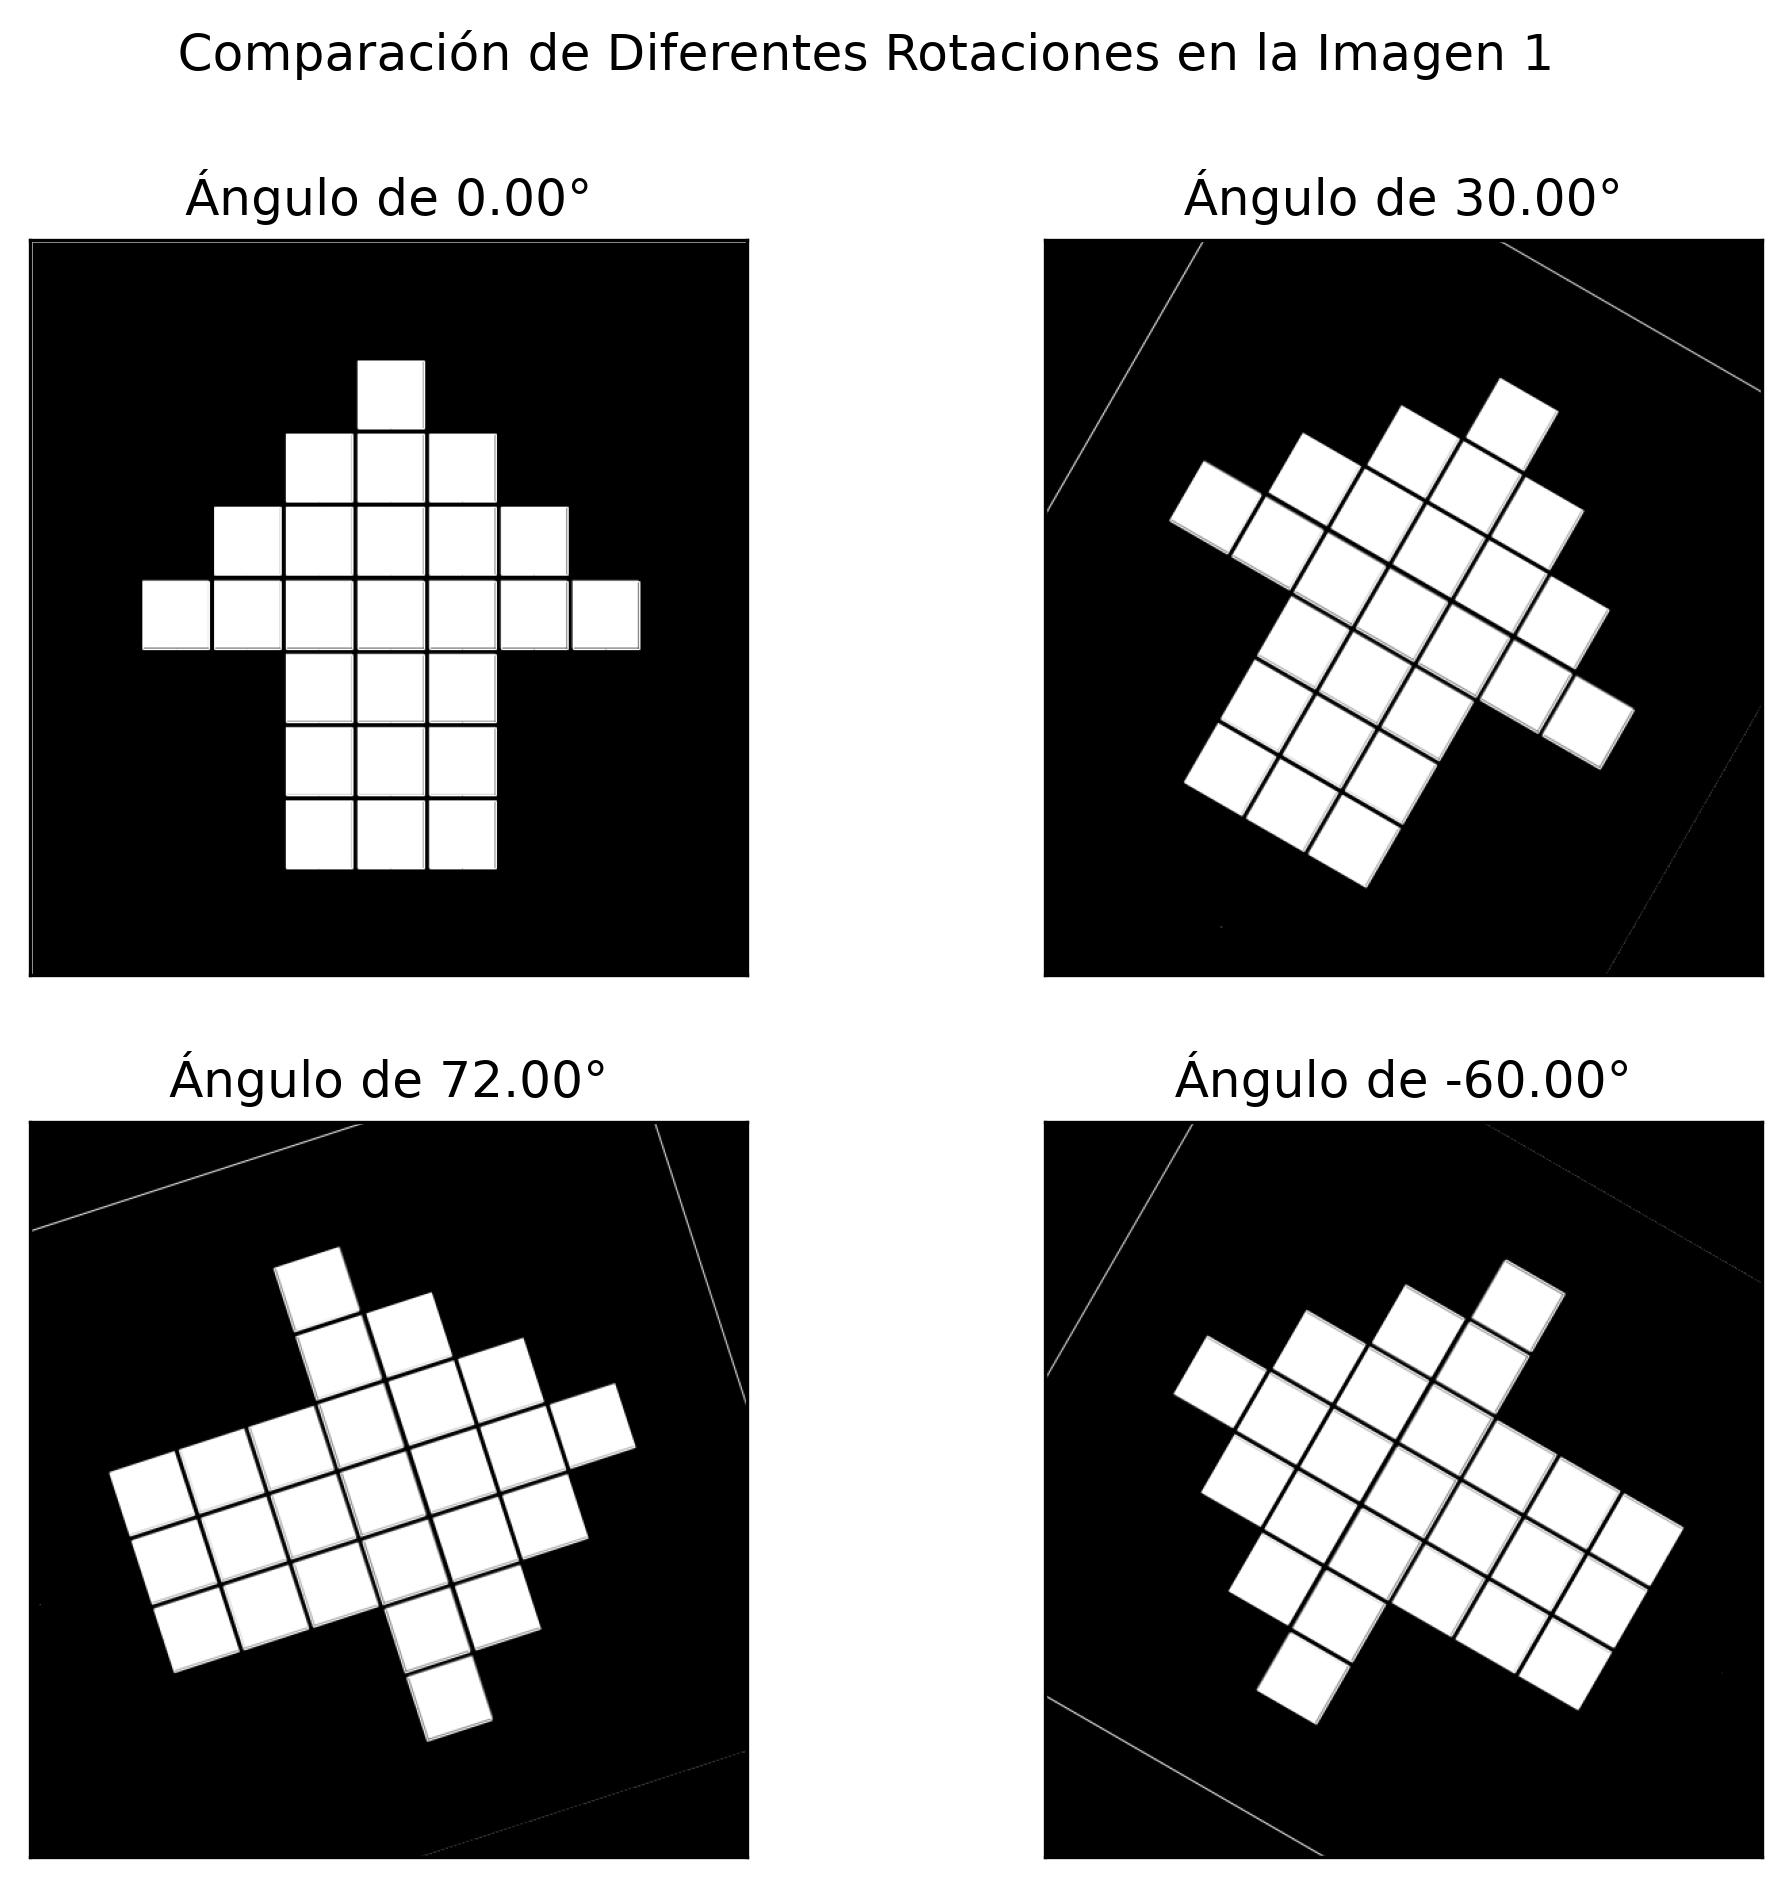
\includegraphics[width=0.65\textwidth]{../results/img_1_rotation.jpg}
            \caption{Diferentes rotaciones centradas de la imagen 1}
        \end{figure}

        Por como se implementó la matriz de rotación, esta se aplica en sentido 
        horario, siendo el sentido natural que uno esperar al rotar un objeto 
        de forma digital. 

    \subsection{Imagen 2 (Traslación)}
        El aplicar diferentes traslaciones a un imagen nos permite observar como 
        se crean ``recortes'' debido a una perdida de información de la imagen. 
        Estos recortes es el resultado esperado de una traslación, debido a que 
        estamos moviendo la ``caja de visión'' de la imagen.

        \begin{figure}[H]
            \centering
            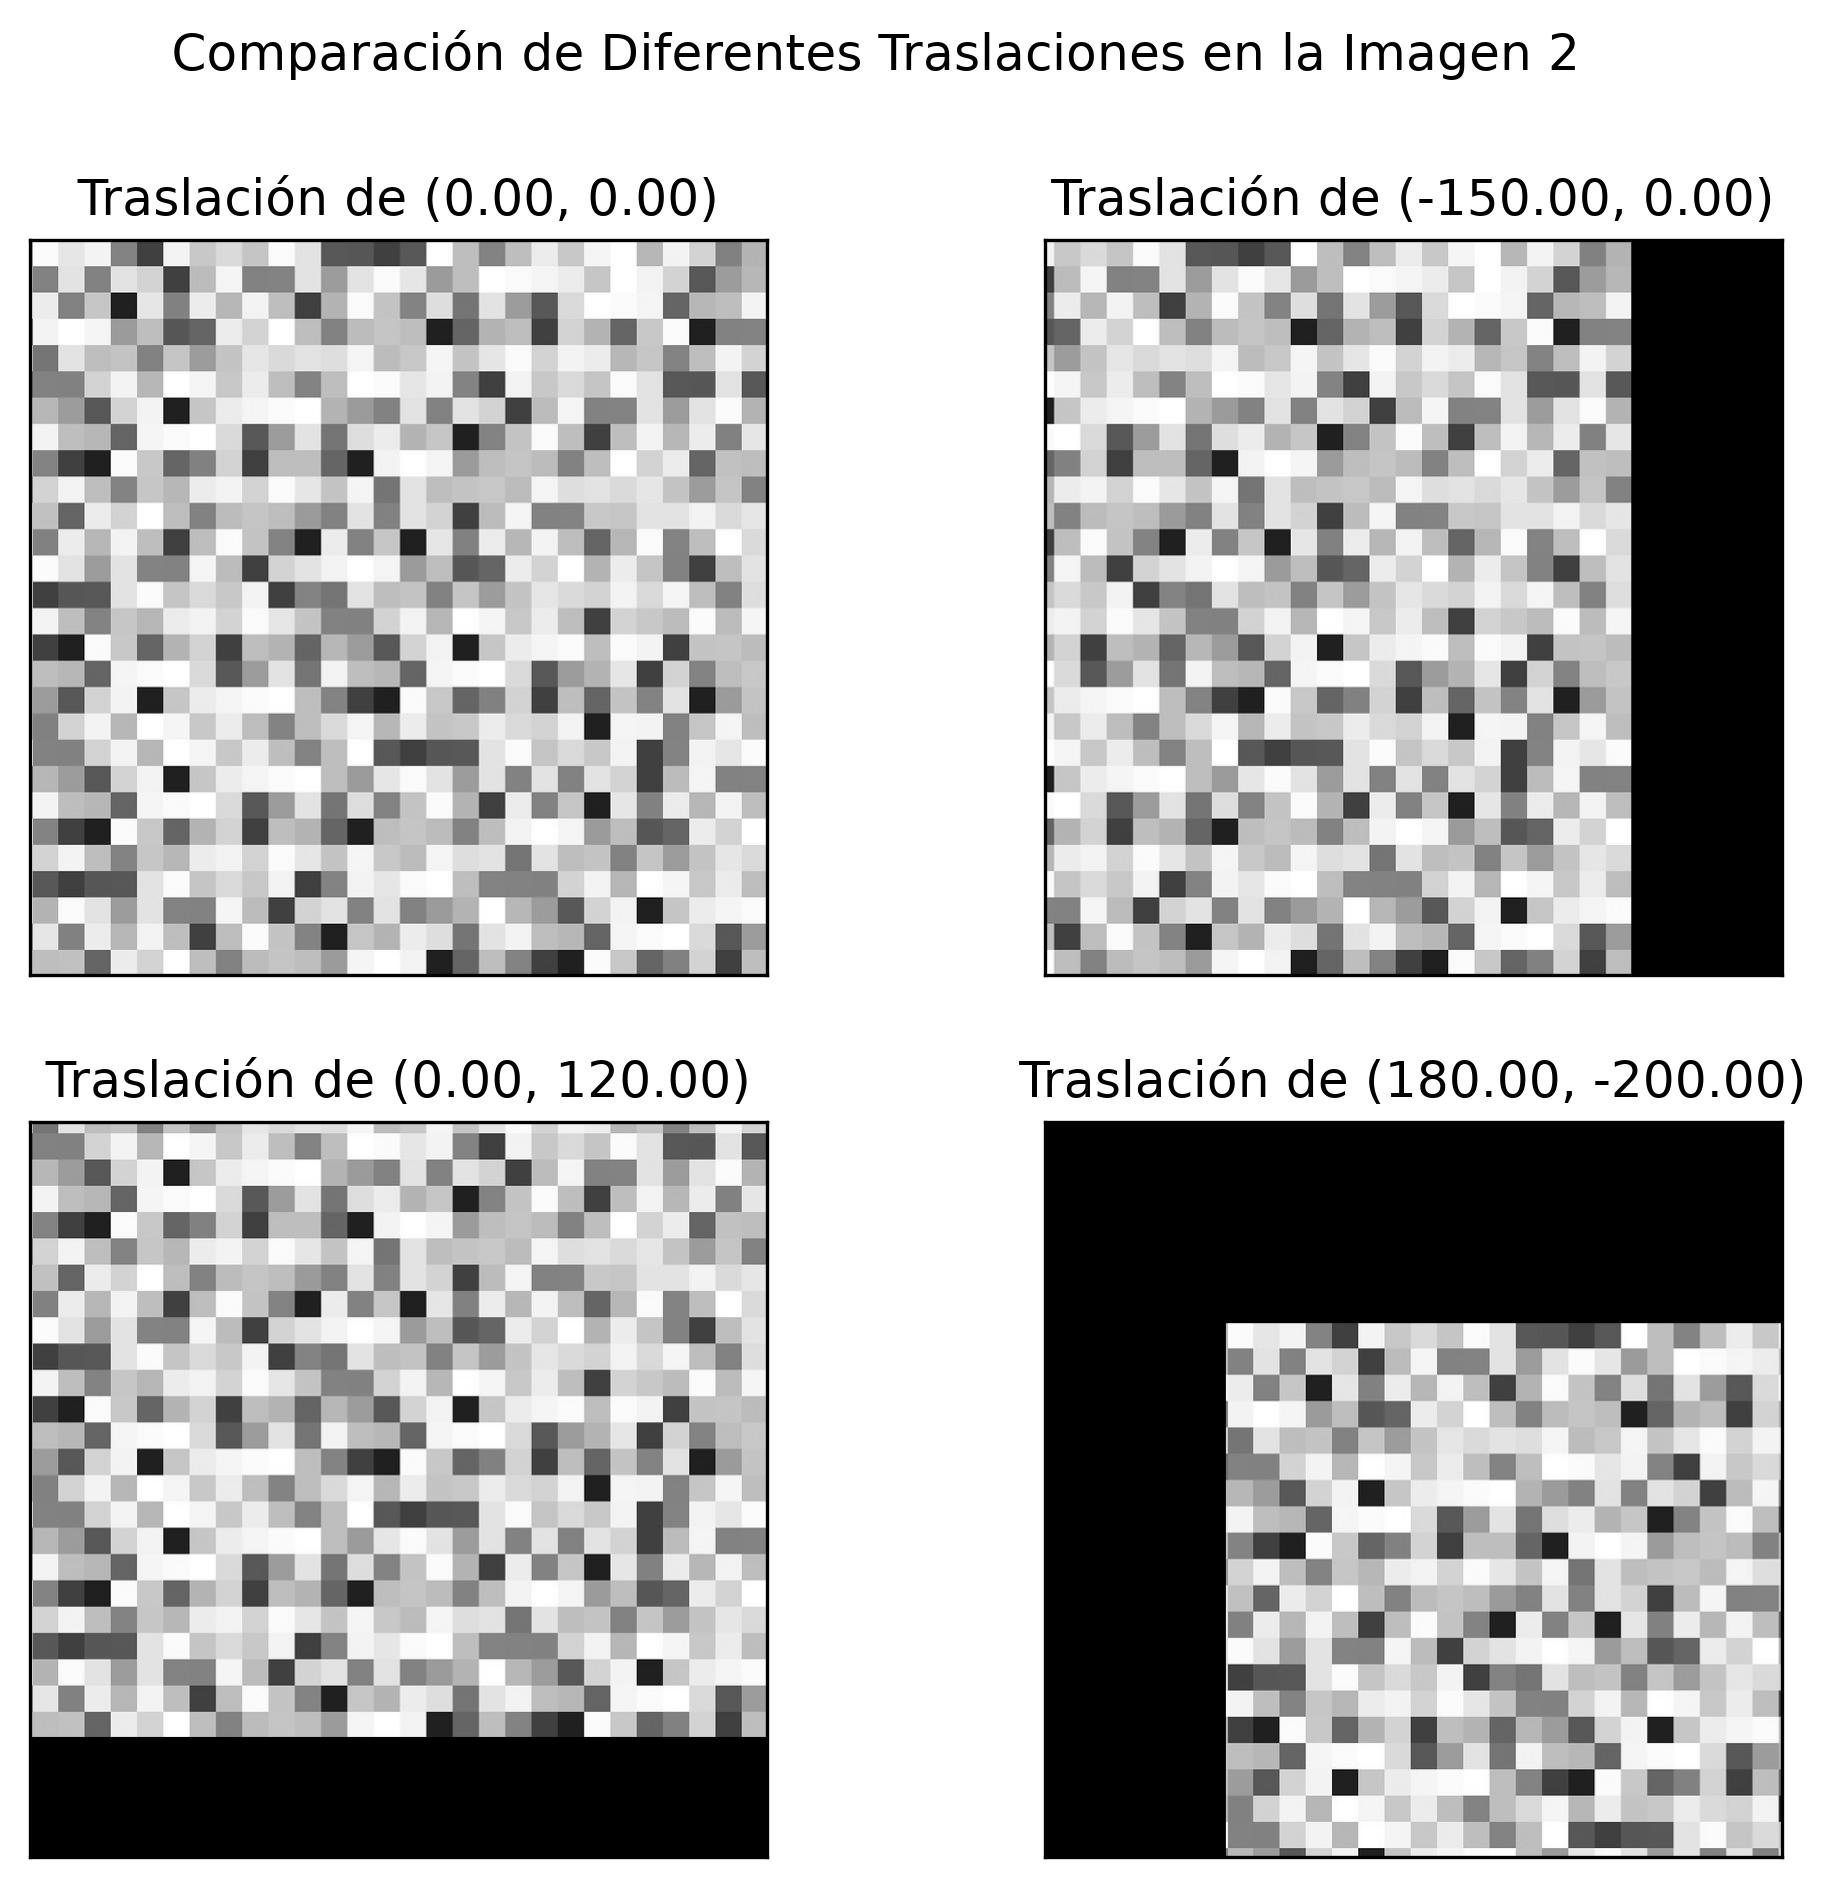
\includegraphics[width=0.65\textwidth]{../results/img_2_translation.jpg}
            \caption{Diferentes traslaciones de la imagen 2}
        \end{figure}

        Por como se implementó la traslación, se tiene que el origen del movimiento 
        es la esquina inferior izquierda, esto para que la imagen esté en el primer 
        cuadrante de un hipotético plano cartesiano.

    \subsection{Imagen 3 (Reflexión)}
        El aplicar la reflexión sobre los ejes centrados a la imagen, se puede 
        observar como la imagen sufre de un efecto ``espejo'' sobre los elementos 
        que la componen. 

        \begin{figure}[H]
            \centering
            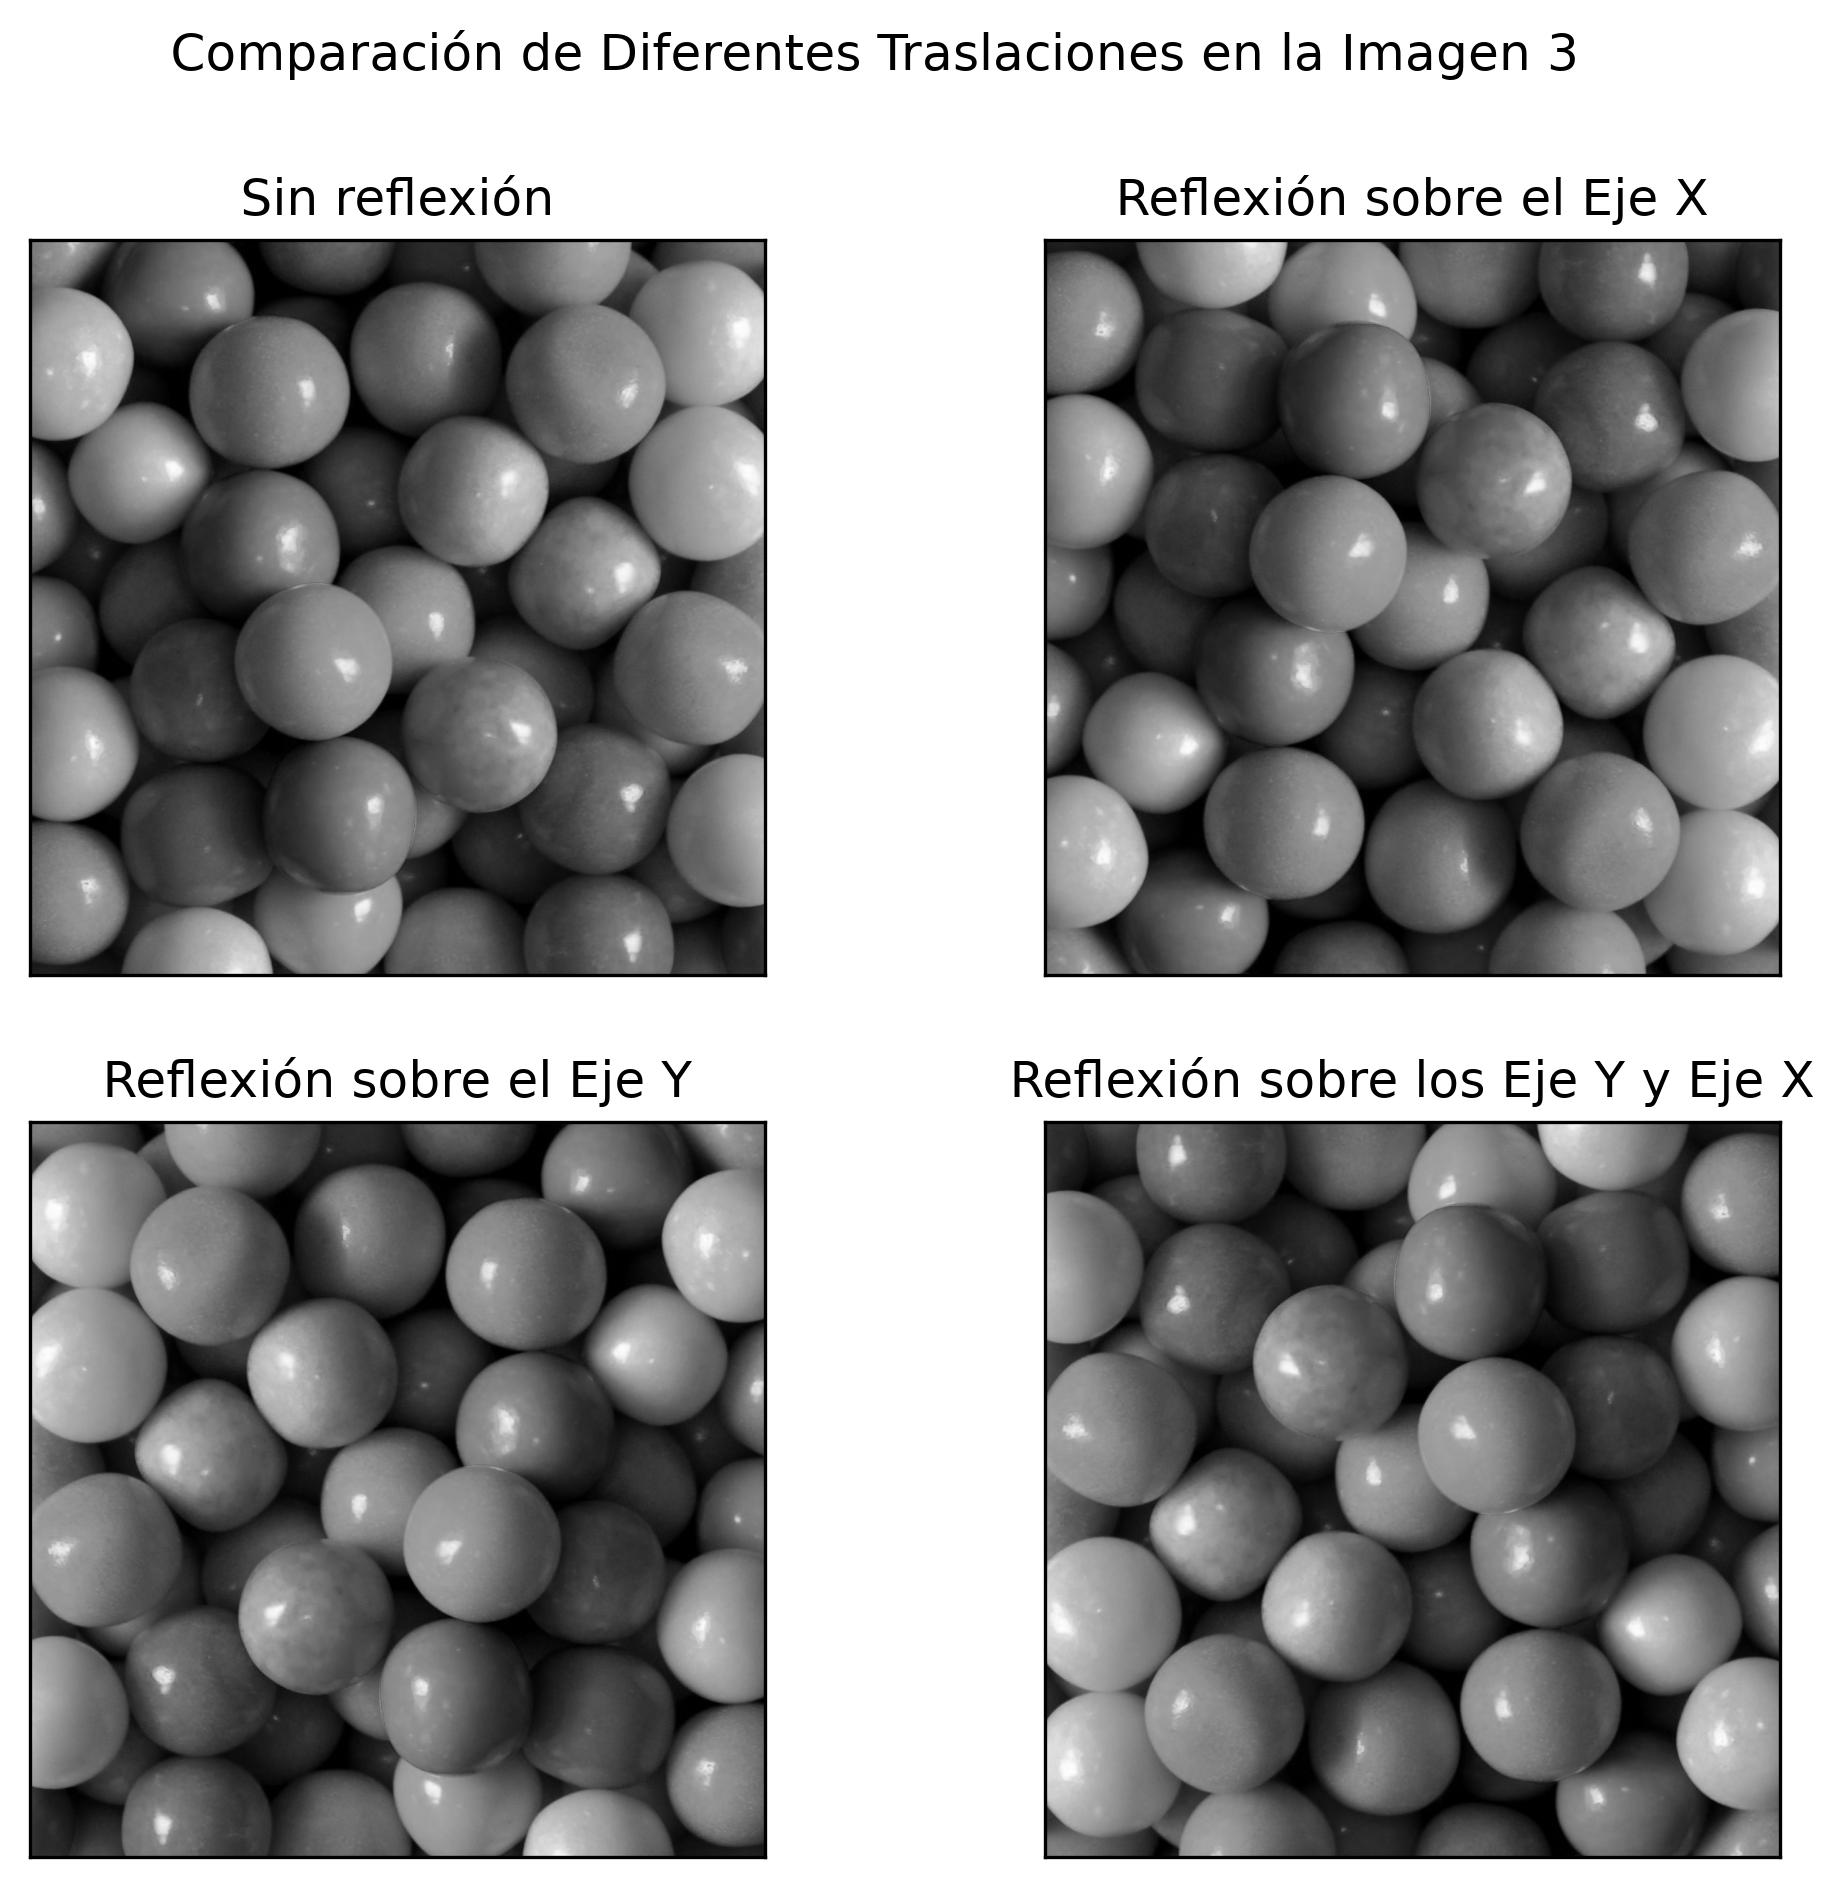
\includegraphics[width=0.65\textwidth]{../results/img_3_reflection.jpg}
            \caption{Diferentes reflexiones de la imagen 3}
        \end{figure}

        Por como se implementó la reflexión, los ejes están invertidos entre cómo se 
        representa la imagen en matriz y cómo se ve en gráfica, pero este un detalle 
        menor que no afecta el resultado final de la transformación.

    \subsection{Imagen 4 (Escalamiento)}
        Escalar la imagen sobre los diferentes ejes de la imagen se puede 
        mostrar de mejor manera ciertos detalles más minuciosos o pequeños. El 
        único detalle es que la imagen es ``recortada'' hacia el eje que se 
        escala cuando su factor es mayor a 1. 

        \begin{figure}[H]
            \centering
            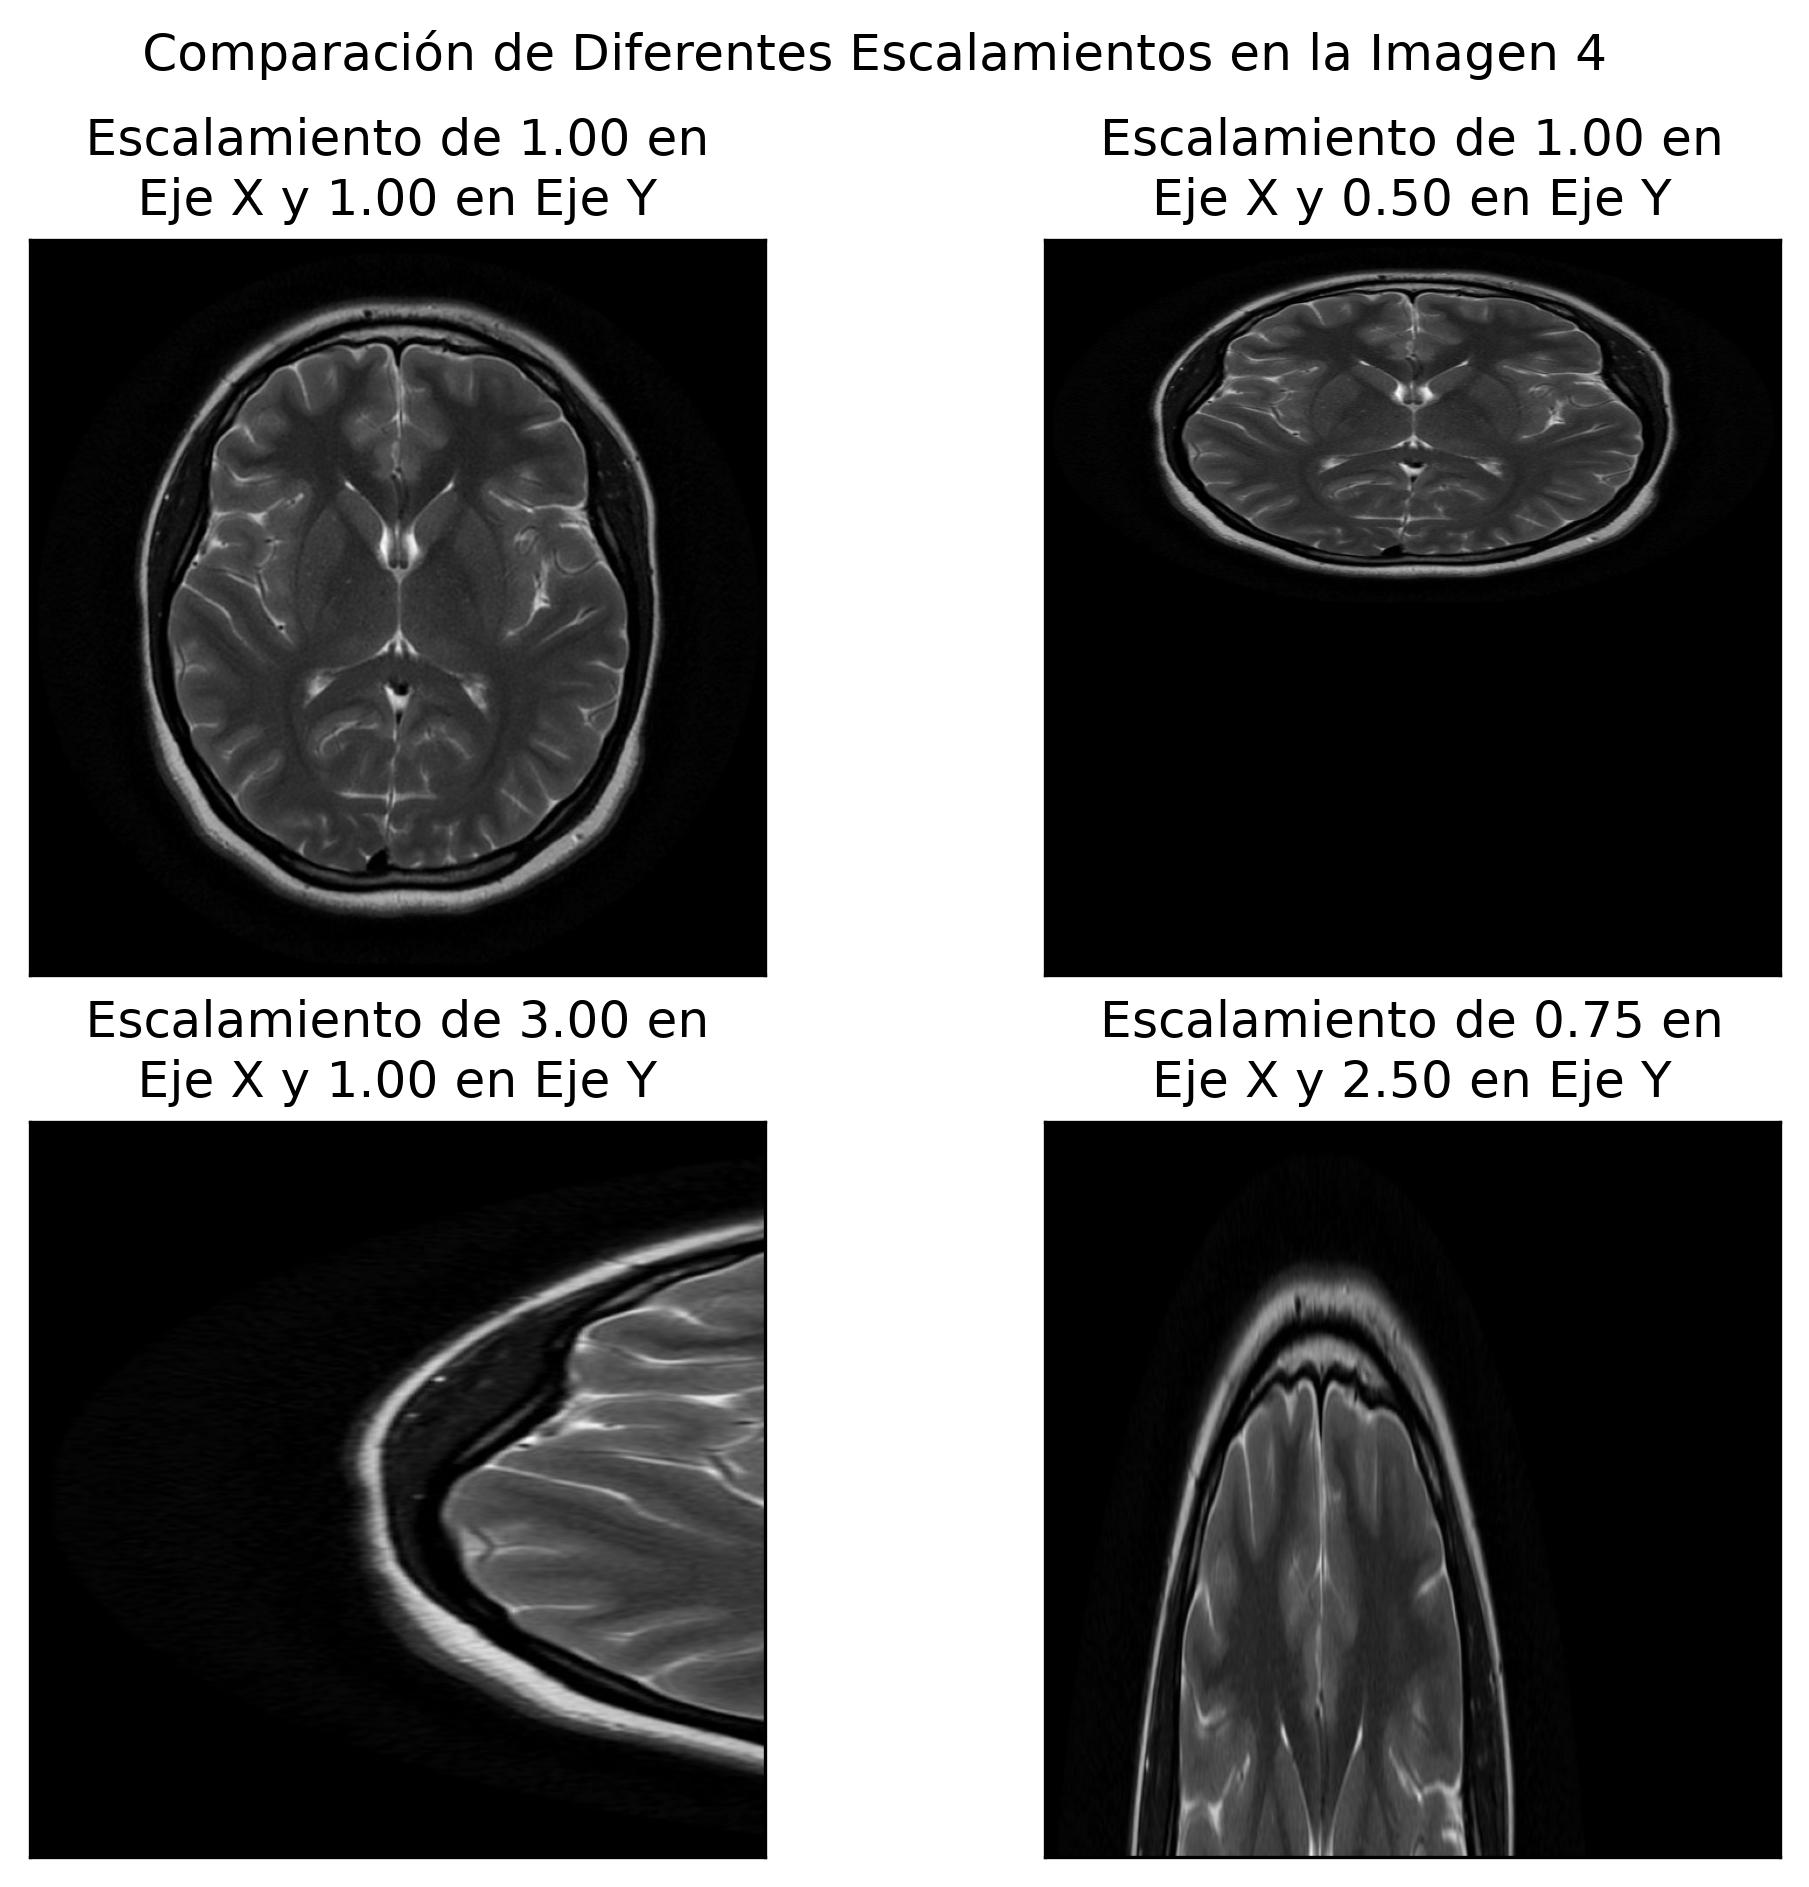
\includegraphics[width=0.65\textwidth]{../results/img_4_scaling.jpg}
            \caption{Diferentes escalamientos de la imagen 4}
        \end{figure}

        Por como se implementó el escalamiento, las entradas del algoritmo está 
        invertidas respectos a los ejes de la imagen y que se generan esos ``recortes'' 
        debido a que la ``caja de imagen'' sigue siendo fija.

    \subsection{Imagen 5 (Transformación Afín)}
        La parte fundamental de las transformaciones afines es componerlas con 
        otras con el propósito de rescatar o mejorar ciertos detalles o elementos 
        presentes en una imagen. Para ilustrar este fenómeno, se presentan algunas 
        composiciones de transformaciones afines:

        \begin{figure}[H]
            \centering
            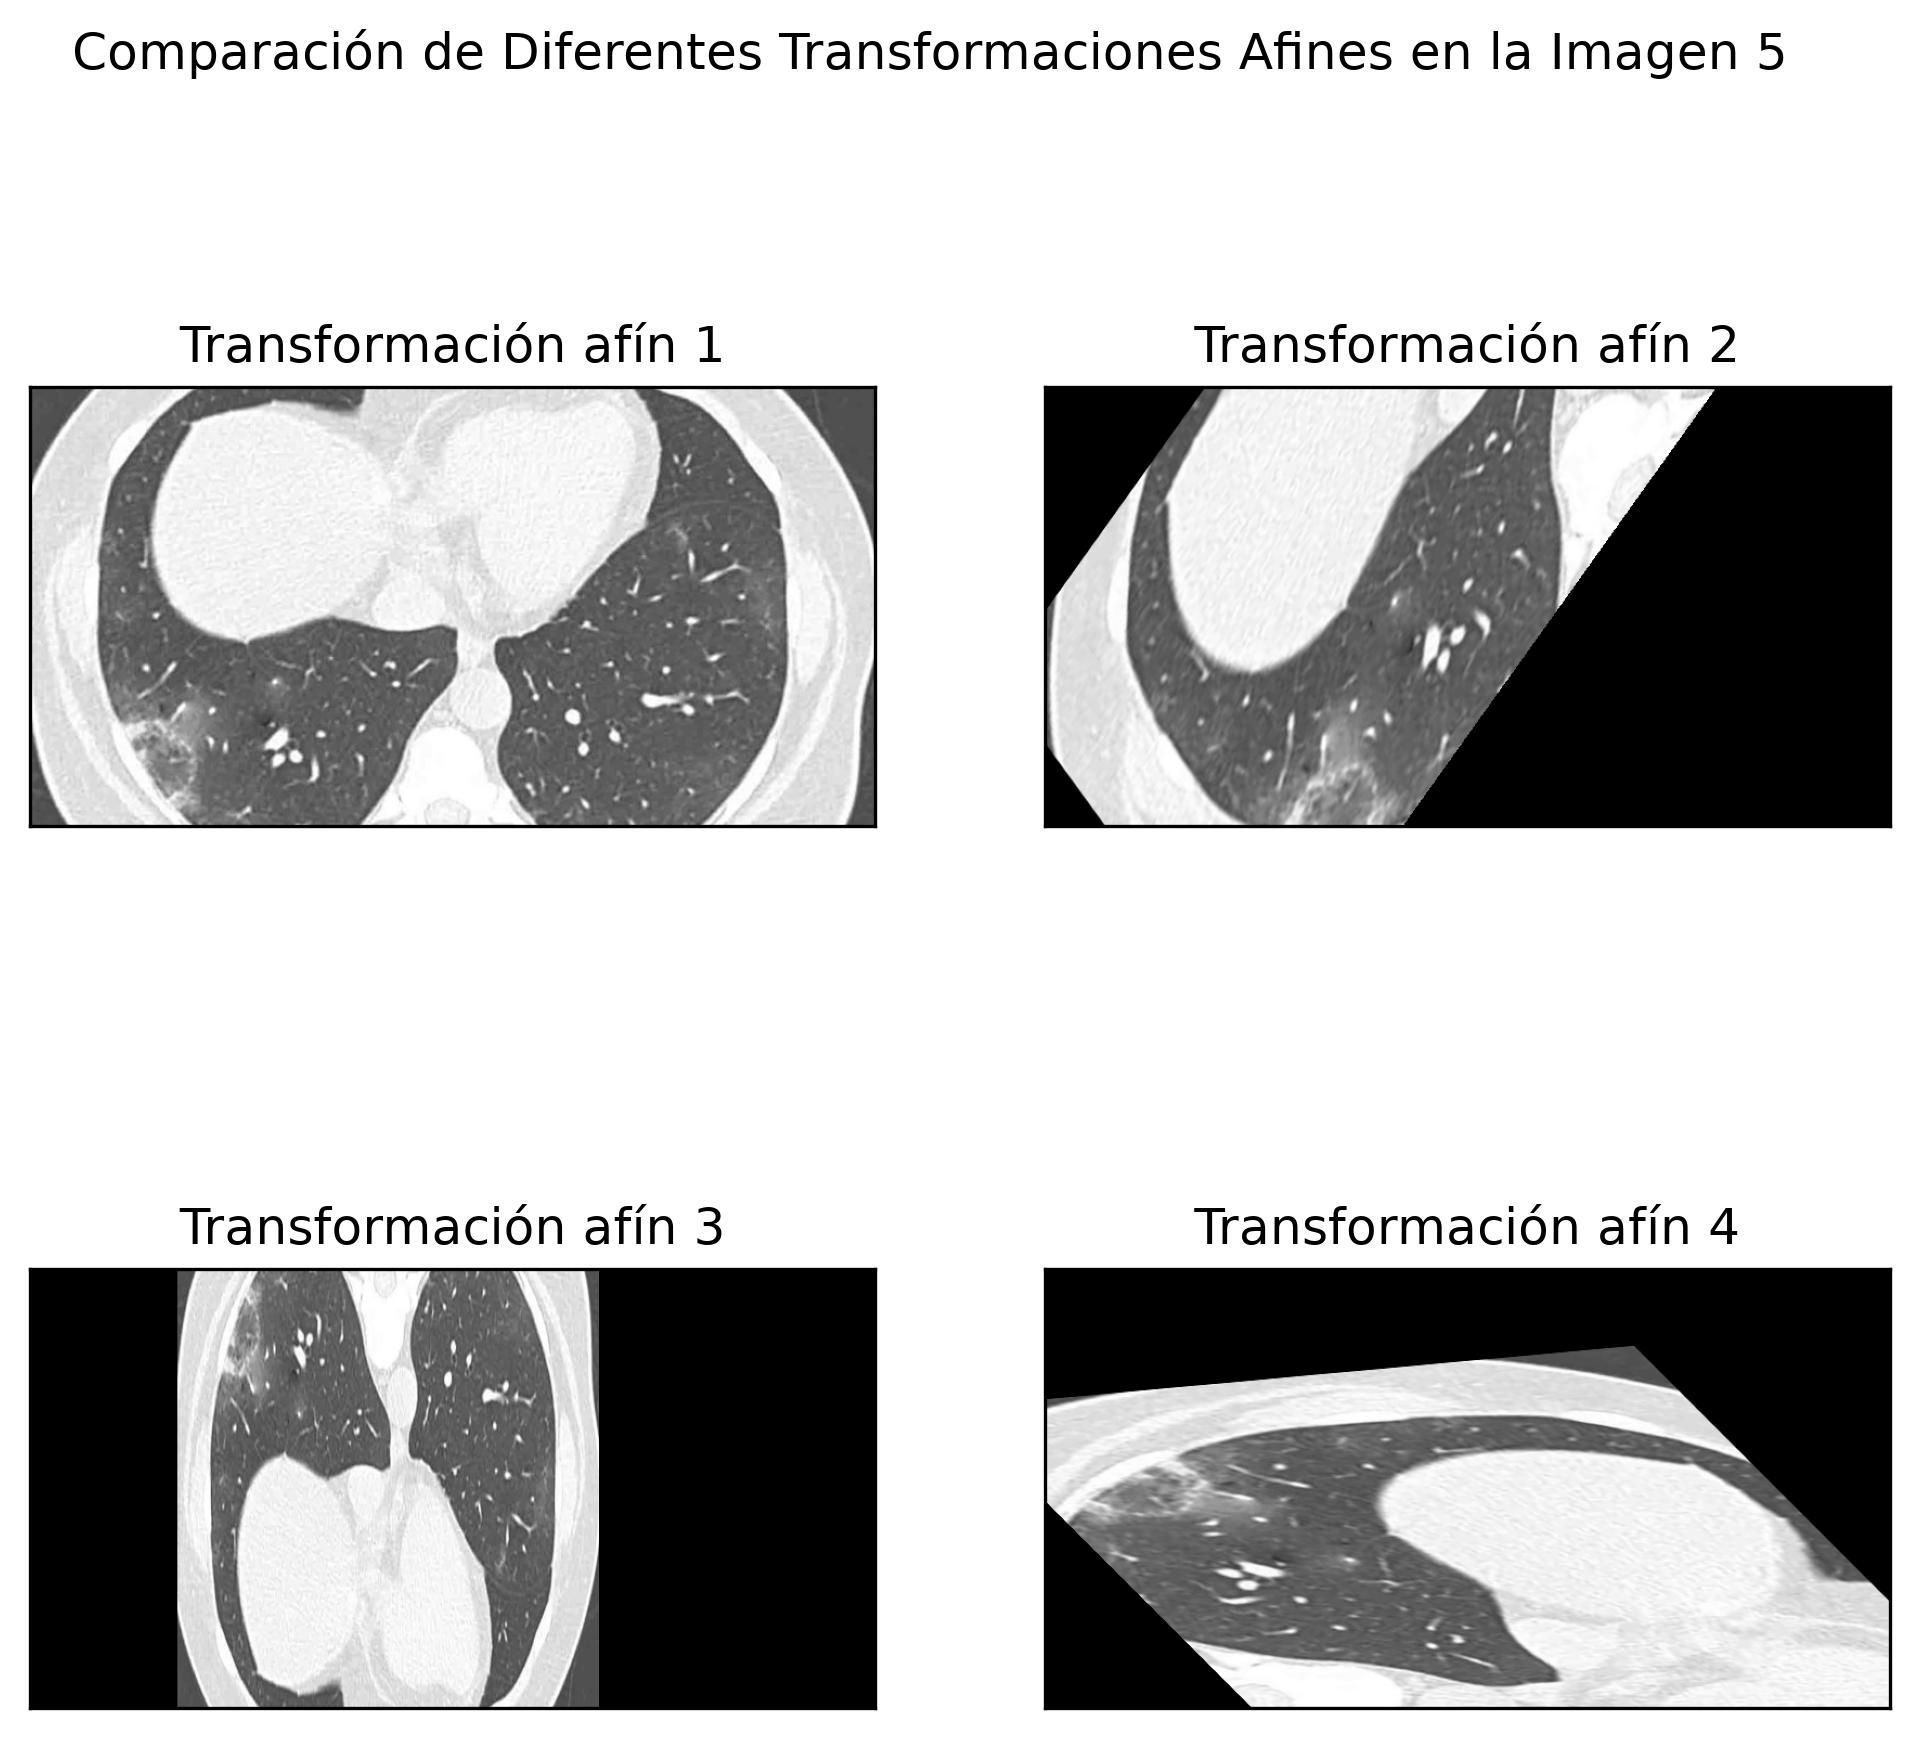
\includegraphics[width=0.65\textwidth]{../results/img_5_affine.jpg}
            \caption{Diferentes transformaciones afines de la imagen 5}
        \end{figure}

        Para lograr los efectos anteriores se emplearon los siguientes parámetros 
        aplicando las transformaciones en el orden cizallamiento, escalamiento, 
        reflexión, rotación y traslación:

        \begin{table}[h]
            \centering
            \begin{tabular}{c | p{9cm}}
                \textbf{Transformación afín} & \textbf{Parámetros} \\ \hline
                1 & Sin transformación afín \\ \hline
                2 & Rotación de $-36°$, escalamiento de $1.5$ en eje X y cizallamiento de $0.5$ sobre el eje Y. \\ \hline
                3 & Traslación de $135$ sobre eje X, reflexión respecto al eje X y escalamiento de $0.5$ en eje X.\\ \hline
                4 & Rotación de $45°$, escalamiento de $1.2$ en eje Y y cizallamiento de $1$ sobre el eje X.\\ \hline
            \end{tabular}
        \end{table}